\chapter[Introduction]{Introduction}

Graphene, a two-dimensional atomistically thin allotrope of carbon, has attracted significant attention from the scientific community following the first unambiguous demonstration of the isolation of monolayer graphene by Andre Geim and Kostya Novoselov at the University of Manchester in 2004\cite{geim_rise_2007, geim_graphene_2009}. The specific arrangement of carbon atoms in the graphene lattice leads to interesting physical, chemical and electrical properties, which multiple groups have exploited for applications in a broad spectrum of domains\cite{berman_few_2013,chen_oxidation_2011, cui_cautionary_2017, su_impermeable_2014, berry_impermeability_2013, hayatdavoudi_mechanistic_2017} ranging from electronics\cite{moreno_bottom-up_2018, fan_graphene_2019,sun_graphene_2010, kim_graphene-contact_2012, avouris_graphene_2010, baeumer_ferroelectrically_2015, bao_atomic-layer_2009,blake_graphene-based_2008, trung_graphene_2022,wang_transparent_2008, liu_ultratransparent_2017, shin_stretchable_2019,kim_large-scale_2009, polat_graphene_2014, anagnostopoulos_mechanical_2016,bae_roll--roll_2010, khan_graphene_2017} to biological applications\cite{akinwande_large-area_2015,lalwani_two-dimensional_2013,mohanty_graphene-based_2008,ohno_label-free_2010,chen_electronic_2012,he_graphene_2010}. The construction of the lattice from C-C $\sigma$-bonds results in the high tensile strength and chemical stability of the graphene lattice.\cite{booth_macroscopic_2008, lee_measurement_2008} In recent years graphene has also found applicability as a suitable membrane for desalination. This is  in part due to the ability to selectively tune the inter-layer spacing among graphene layers. Such inter-layer tuning alters the dynamics of water molecules and salt ions passing through the nanochannels.\cite{abraham_tunable_2017, nair_unimpeded_2012, gopinadhan_complete_2019, radha_molecular_2016, saini_selective_2022, yang_self-assembly_2018, paechotrattanakul_ultrahigh_2023, gao_confined_2022, gao_graphene_2022}

In addition to the above mentioned properties graphene provides a large surface area which facilitates the adsorption of molecules to enable self-assemblies. The adsorption of molecules on graphene is driven by hydrophobic interactions with the graphene lattice and interactions with the large electron cloud above the graphene surface formed by the presence of unhybridized $p_z$ orbital at every carbon site. The transparency of graphene also allows for real-time monitoring of the self-assembly processes, making graphene an attractive two-dimensional substrate.\cite{xu_coadsorption_2006, zhao_investigating_2016, hason_arrangements_2023, xu_directional_2021, garah_guanosine-based_2015, hughes_adsorption_2017, hassan_interactions_2014, hsun_su_electrostatic_2011} 

Self-assembly of molecules over a graphene surface can be classified by the interactions driving the process:
\begin{itemize}
    \item Self-assemblies driven by hydrophobic interactions, as observed in the case of benzene\cite{alzahrani_first-principles_2010,shen_adsorption_2021,hassan_interactions_2014,wang_substituent_2014}, naphthalene and fullerenes\cite{lu_using_2012}.
    \item Self-assemblies driven purely by electrostatic interactions, as observed in the case of positively charged Fe\textsubscript{3}O\textsubscript{4} on negatively charged graphene oxide\cite{yang_electrostatic_2020}, graphene-ion intercalations\cite{lee_li_2012,yoon_chloroaluminate_2022,yu_reversible_2023,ji_lithium_2019} and other structures\cite{groger_step-wise_2009}. 
    \item Self-assemblies driven by both hydrophobic and electrostatic interactions, as observed in nucleobases\cite{heckl_two-dimensional_1991,freund_structure_1997,mu_temperature-dependent_2013,gottarelli_self-assembly_2000,ciesielski_nanopatterning_2010}, organic acids\cite{rochefort_interaction_2009,griessl_self-assembled_2002}, polar organic molecules\cite{song_noncovalent_2016,su_composites_2009} and phthalocyanines\cite{jarvinen_self-assembly_2014,hamalainen_self-assembly_2012}.
\end{itemize}

\begin{figure}[h]
    \centering
    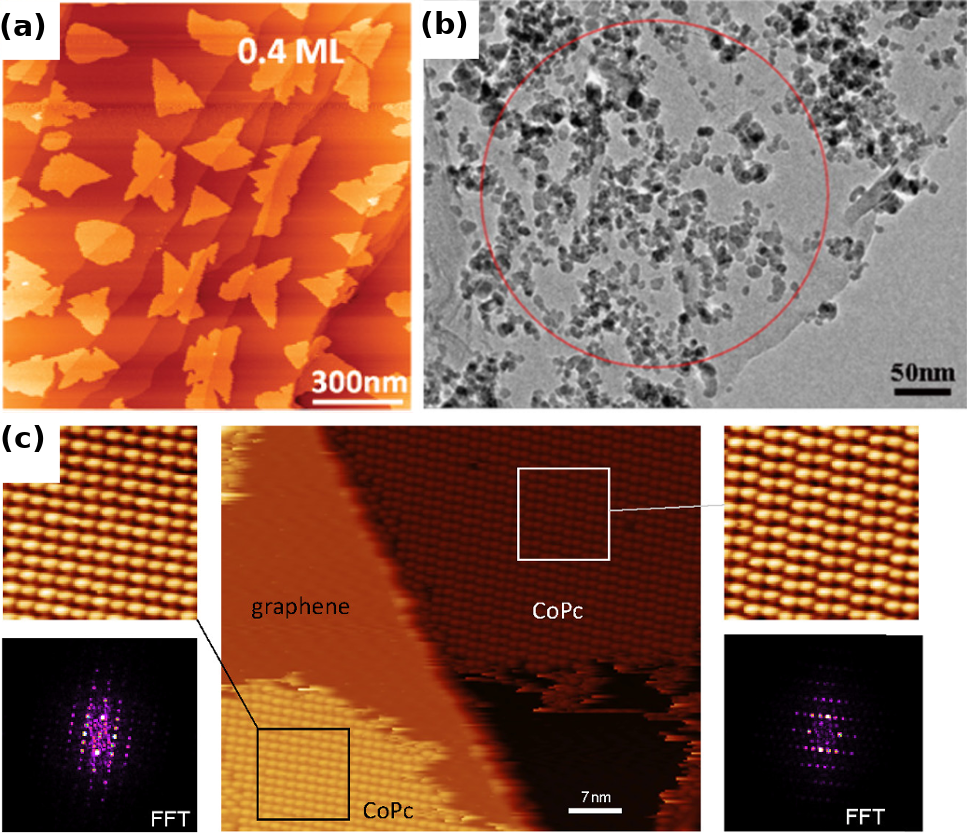
\includegraphics[width=0.8\textwidth]{Introduction/Figures/Untitled_new.png}
    \caption[Representative images depicting various types of self-assemblies formed over a graphene surface]{(a) STM image showing dentritic growth of C\textsubscript{60} islands on graphene/Ru(0001) at low coverage. Reprinted (adpated) with permission from ref.\supercite{lu_using_2012}. Copyright 2023 American Chemical Society. (b) TEM image of 10Fe-GO system. Reprinted (adapted) with permission from ref.\supercite{yang_electrostatic_2020}. (c) STM image (0.7V/2pA) showing two CoPc islands with kinks in different directions of the CoPc lattice. Reprinted (adapted) with permission from ref.\supercite{hamalainen_self-assembly_2012}. Copyright 2023 American Chemical Society.}
    \label{fig:enter-label}
\end{figure}

We briefly illustrate each of the interactions with salient examples. Molecules which are devoid of H-bonding groups or ionic groups and contain only hydrophobic cores self assemble over the graphene surface by hydrophobic driven interactions. An example of this is the self assembly of fullerene (C60) over the graphene surface. Loh and coworkers employed STM imaging to investigate the self-assembly of C\textsubscript{60} over a graphene/Ru(0001) substrate.\supercite{lu_using_2012} They chose graphene/Ru(0001) substrate due to the formation of corrugated structures, which could then influence the formation of C\textsubscript{60} self-assemblies. At low surface coverage, they observed that the C\textsubscript{60} molecules would preferentially occupy the C\textsubscript{hcp} valleys, the remaining molecules would undergo a hierarchical adsorption with the C\textsubscript{fcc} valleys getting filled next, followed by the highest points in the corrugations and finally six C\textsubscript{60} molecules would occupy the periphery of the corrugations [Figure 1.1(a)]. 

Metals and metallic nanoparticles interact with the graphene surface via electrostatic interactions. Shuai and coworkers investigated the assembly of \textit{p}-Fe\textsubscript{3}O\textsubscript{4}.\supercite{yang_electrostatic_2020}  They observed that the positively charged Fe\textsubscript{3}O\textsubscript{4} particles would form self-assemblies over the negatively charged graphene oxide (GO) via electrostatic interactions. From TEM images, they confirmed that the \textit{p}-Fe\textsubscript{3}O\textsubscript{4} nanoparticles were able to form homogeneous assemblies over GO nanosheets, in the case of 10Fe-GO system [Figure 1.1(b)]. They also observed that the electrostatic interactions between the positively charged Fe\textsubscript{3}O\textsubscript{4} particles and the negatively charged GO sheets have a synergic effect, promoting the dispersion of both the structures.

Molecules which contain a chelated metal, exhibit both electrostatic and hydrophobic interactions with the graphene sheet. Sainio and colleauges investigated the formation of self-assembled monolayers in Cobalt-Phthalocyanines over a graphene/Ir(111) substrate using STM imaging.\supercite{hamalainen_self-assembly_2012} They observed that the CoPc molecules formed a square lattice over the graphene surface [Figure 1.1(c)], even though the underlying graphene/Ir(111) moire pattern had a hexagonal symmetry. They concluded that this was due to the weak coupling between the graphene and the underlying Ir(111) surface, and opined that graphene/Ir(111) can be a suitable substrate to further investigate the formation of molecular self-assemblies.

Molecules which exhibit extended self-assembled stcutures are those which contain H-bond donor and acceptor groups. Nucleic acids are known to form extendes self assemblies on metallic surfaces like Au(111) and and Cu(111).\supercite{kelly_understanding_2008,lukas_adenine_2009,tsud_adenine_2015,otero_guanine_2005,otero_elementary_2008} Besenbacher and coworkers investiagted the formation of self-assembled monolayers in canonical nucleobases dispersed over Au(111) using STM imaging and ab-initio modelling.\supercite{kelly_understanding_2008,lukas_adenine_2009,otero_guanine_2005,otero_elementary_2008} They observed the formation of ordered networks at low surface coverages which gradually transformed towards random glassy structures with increasing surface coverages.\supercite{otero_elementary_2008}  Nucleobases are also found to form self assemblies on graphene surfaces. Multiple groups have investiagted the formation of 2D self-assemblies in nucleobases dispersed over a graphene surface.\supercite{heckl_two-dimensional_1991,freund_structure_1997,xu_coadsorption_2006,akinwande_large-area_2015,spada_guanosine-based_2008,mamdouh_supramolecular_2006} Heckl and colleagues investigated the formation of 2D networks in adenine molecules dispersed over a graphite surface using STM imaging and Low Energy Electron Diffraction (LEED) experiments.\supercite{heckl_two-dimensional_1991} Similar studies were performed for other nucleobases and (or) nucleobase derivatives.\supercite{freund_structure_1997,xu_coadsorption_2006,mamdouh_self-assembly_2009,wang_controlling_2014,mu_temperature-dependent_2013} The adsorption of nucleobases on the graphene surface is mediated by $\pi-\pi$ interactions, and the preferred orientation of the adsorbent molecule is to align parallel to the underlying graphene surface in order to maximize the $\pi-\pi$ interactions between them. The adsorbent molecules also prefer a ‘AB’ type stacking with respect the underlying graphene lattice, where the face of the adsorbent molecule is slightly shifted from the graphene lattice.

In addition to the self assembly of nucleobases on graphene polymeric DNA strands are also know to adsorb and undergo 2D diffusion over graphene surfaces.\supercite{hampitak_protein_2020,wei_control_2019,he_planar_2020,shankla_step-defect_2019,shankla_conformational_2014,wells_assessing_2012} One of the unique features of multilayer graphene is the interlayer spacing of $\approx$ 3.4 ang. This matches the distance between subsequent nucelobases (rise) observed in DNA. These features attracted the exploration of graphene based solid state nanopores for sequencing DNA. In 2010, three groups independently demonstrated the applicability of graphene membranes as suitable tools to detect DNA translocations.\supercite{merchant_dna_2010,schneider_dna_2010,garaj_graphene_2010} They were able to drive the DNA strand through a nanopore constructed in the graphene membrane, and used blockades in the ionic current flowing across the membrane to identify the translocation of DNA strands. This indicated the possibility of employing graphene-based solid-state devices to sequence DNA strands. Solid-state nanopores, such as those constructed in graphene, can sequence long single-stranded DNA molecules without requiring strand fragmentation.\supercite{merchant_dna_2010,schneider_dna_2010,garaj_graphene_2010,li_dna_2003,yuan_solid-state_2018,xue_solid-state_2020} The fragmentation of the full DNA into overlapping short segments is a required step in traditional Sanger-based methods used in many next-generation sequencing methods, and it is a common source of error in reconstructing the complete DNA sequence.\supercite{sanger_dna_1977,daniels_sanger_2021,curci_how_2015} Therefore, it is imperative that a clear understanding of the dynamics of DNA strands near graphene nanopores is required to design graphene membranes with specific properties for DNA sequencing.\supercite{schneider_tailoring_2013}. As a first step towards that, it is critical to understand the interactions between the nucleobases, nucleosides, and nucleotides and the graphene surfaces.

Here, we summarize the experimental and theoretical studies describing the interaction of nucleic acids, both as an individual nucelobase and as a polymer, with graphene. We categorize the results in two broad areas: (a) Graphene as a two-dimensional solid support for nucleobase-assisted self-assemblies and (b) Graphene based nanopores as a reliable tool for rapid sequencing of DNA. 

The Introduction is organized in the following order:
\begin{itemize}
    \item We first discuss the studies describing the binding energetics of monomeric nucelobases or polymeric DNA strands interacting with the graphene surface.
    \item We then focus on the formation of nucleobase self-assemblies over a graphene surface.
    \item In the final section, we review the studies utilizing graphene-based devices for sequencing single-stranded DNA (ssDNA) and double-stranded DNA (dsDNA).
\end{itemize} 

In all the sections we discuss results from both the experimental and theoretical standpoints.

\section{Energetics of Interactions with Graphene surface}
The interaction between the nucleobases and the graphene surface has been investigated in the literature via experimental and computational studies. Isothermal calorimetry (ITC)  experiments and single-molecular force spectroscopy (SMFS) are employed to investigate the binding of nucleobases and (or) short ssDNA strands with the graphene surface. We note that ab-inito DFT calculations generally employ the following scheme to obtain the binding energies and minima, where a routine geometry optimization is performed for the combined nucleobase - graphene model system, and the binding energies are then obtained as the difference between the energy of the nucleobase - graphene system and the sum of individual molecules (graphene sheet and nucleobase). On the other hand, Molecular Dynamics (MD) simulations generally adopt a metadynamics pathway for the investigation of such binding energies, where a particular reaction coordinate, generally denoted as $\zeta$ (the z-projected distance between the nucleobase and the graphene surface in this case) is scanned in an MD simulation via the application of a biasing force. Here, we review a few critical experimental and computational studies investigating the vdW interactions between the nucleobases (small DNA strands) with the graphene surface.

\subsection{Nucleobases}
\subsubsection{Experimental Studies}
\paragraph{Isothermal calorimetry:}To understand the interactions between nucleobases and graphene surface, Rao and coworkers investigated the binding free energies of four canonical DNA nucleobases with the graphene surface using isothermal calorimetry (ITC) experiments in aqueous and basic environments.\supercite{varghese_binding_2009} They obtained an interaction energy of -6.64 (-11.85), -- (-13.45), -4.39 (-9.38) and -0.68 (-4.72) kcal/mol for adenine, guanine, cytosine and thymine in aqueous (basic) environments. The binding free energies obtained by Varghese et al. follow the relative ordering of guanine $>$ adenine $>$ cytosine $>$ thymine, with significantly stronger interactions with the graphene surface in basic media compared to aqueous media.

\subsubsection{Computational Studies}
\begin{figure}
    \centering
    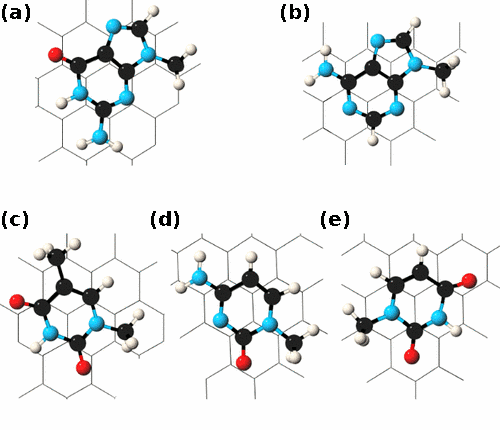
\includegraphics{Introduction/Figures/Figure2.png}
    \caption[Equilibrium geometry of nucleobases on top of graphene: (a) guanine, (b) adenine, (c) thymine, (d) cytosine, and (e) uracil from ab-initio calculations]{Equilibrium geometry of nucleobases on top of graphene: (a) guanine, (b) adenine, (c) thymine, (d) cytosine, and (e) uracil. Reprinted (figure) with permission from S. Gowtham, Ralph H. Scheicher, Rajeev Ahuja, Ravindra Pandey, and Shashi P. Karna, Physical Review B, 76, 033401, 2007.\supercite{gowtham_physisorption_2007} Copyright 2023 by the American Physical Society.}
    \label{fig:enter-label}
\end{figure}
\paragraph{ab-initio studies:} Karna and coworkers investigated the structure and interaction energies for nucleobases over a graphene surface to better understand the various factors influencing the physisorption of nucleobases over the graphene surface.\supercite{gowtham_physisorption_2007} They employed periodic density functional theory (DFT) and single molecule calculations at M\"{o}ller-Plusset (MP2) level of theory and split-valence 6-311++G(d,p) basis set to investigate the relevant descriptors. They observed that interaction energies are dependent on the orientation of the nucleobases with the graphene surface, with parallel stacking of nucleobases being the most stable configuration [Figure 1.2]. They also observed that the presence of heteroatoms (nitrogen and oxygen) on the nucleobases affects the interactions between the nucleobases and the graphene surface. The binding energies obtained for adenine, guanine, cytosine, thymine and uracil are -21.68, -24.68, -18.45, -19.14 and -17.06 kcal/mol, respectively. They also observed a strong dependence on the molecular polarizability of the nucleobases on the stabilization of the inter-molecular interactions, with guanine having the highest molecular polarizability and uracil having the lowest molecular polarizability.

Grimme and coworkers investigated the structure and interaction energies of stacked graphene nucleobase complexes.\supercite{antony_structures_2008} They employed DFT calculations at B97-D functional and a triple-zeta valence plus polarization TZV(2d,2p) basis set to investigate the relevant properties of the complexes (interaction energies, geometries and electronic properties). They found that interaction energies strongly depend on the stacking geometry. The most stable configuration is the parallel stacked configuration, which maximizes the $\pi$-stacking interactions between the graphene surface and the nucleobase. The binding energies for adenine, guanine, cytosine, thymine and uracil were calculated to be -20.6, -26.3, -19.2, -19.9 and -17.0 kcal/mol, respectively, for graphene. They also observed that the interactions between the graphene surface and the nucleobases are primarily mediated via dispersion interactions, and the interaction energies show a direct relationship with the number of carbon atoms included in the graphene unit cell, with approximately 50 atoms required to reach convergence in cases of nucleobase interactions.
\begin{figure}
    \centering
    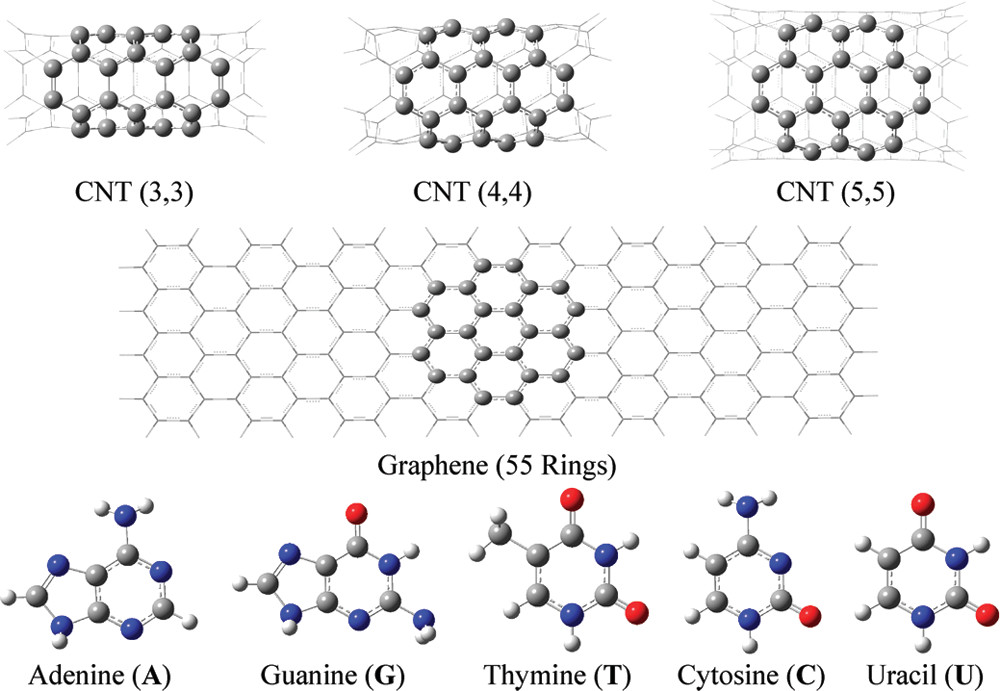
\includegraphics{Introduction/Figures/Figure3.png}
    \caption[Representative structures corresponding to (3,3), (4,4), (5,5) SWCNTs, graphene sheet and canonical nucleobases]{Representative structures corresponding to (3,3), (4,4), (5,5) SWCNTs, graphene sheet and canonical nucleobases. Atoms considered interacting in ONIOM are depicted as balls and sticks, and other atoms are depicted as lines. Figure adapted from ref \supercite{umadevi_quantum_2011}.}
    \label{fig:my_label}
\end{figure}

Using single-molecule DFT calculations, Sastry and coworkers studied the interaction energies for nucleobases over a poly-conjugated surface and carbon nanotubes.\supercite{umadevi_quantum_2011} They investigated the binding energies of nucleobases with four sets of surfaces: a flat graphene surface and three carbon nanotubes of increasing radii starting from (3,3) to (5,5) as shown in Figure 1.3, using ONIOM formalism with M06-2x Minnesota functional and 6-31g* basis set to describe atoms in the QM layer, and AM1 semi-emperical method to describe other atoms. The binding energies obtained for nucleobases interacting with the graphene surface are -14.14, -14.78, -13.30, -14.29 and -11.92 kcal/mol for adenine, guanine, cytosine, thymine and uracil, respectively. They observed that the nucleobases' binding energies strongly depend on the curvature of the surface, with the highest binding energies obtained when the surface is devoid of curvature. This observation was ascribed to the increase in the $\pi$-stacking interactions between the nucleobase and the adsorbent surface as the curvature of the adsorbent decreases.

Kim and coworkers investigated the non-covalent interactions between nucleobases and a graphene surface using DFT calculations.\supercite{cho_noncovalent_2013} They studied the binding of nucleobases with two systems: naphthalene and a graphene surface (modelled as an n=5 flake with 150 carbons arranged in hexagonal symmetry). The authors obtained interaction energies of -19.8, -21.7, -18.4 and -19.7 kcal/mol for adenine, guanine, cytosine and thymine, respectively using periodic DFT calculations at the semilocal Perdew–Burke–Ernzerhof (PBE) functional coupled with the pairwise Tkatchenko-Scheffler (TS) dispersion correction, with guanine having the strongest binding while cytosine being the weakest. We note that the binding free energies obtained by Kim and coworkers are comparable to the values obtained by Karna et al.\supercite{gowtham_physisorption_2007} and Grimme et al.\supercite{antony_structures_2008} while differing in the computational methods adopted.

Cho and coworkers investigated the interaction between nucleobases and graphene surface using DFT calculations\supercite{lee_physisorption_2013}. They evaluated the binding free energies using multiple functionals (LDA, PBE, PBE+vdW and vdW-DF) and observed that guanine had the strongest binding across all nucleobases, while cytosine was the weakest. The authors obtained the binding energies of -23.06 (-14.53), -27.31 (-17.06),  -21.45 (-13.38) and  -21.91 (-13.84) kcal/mol for adenine, guanine, cytosine and thymine, respectively from PBE+vdW (vdW-DF) calculations. They also observed that the the main contribution to the vdW interactions between the nucleobases and the graphene surface arises from the $\pi$-orbitals belonging to the substrate and the nucleobase.

The binding energetics of canonical nucleobases with the graphene surface have also been investigated by other groups using different levels of calculation.\supercite{panigrahi_interaction_2012,cortes-arriagada_intermolecular_2021,cortes-arriagada_phosphorene_2018,le_physisorption_2012} In one such study, Ganguly and coworkers employed M06-2x Minnesota functional with 6-31g(d) basis set to investigate the binding of free nucleobases and a fluorophore tagged version with the graphene surface\supercite{bhai_probing_2020}. The authors observed that the binding free energy followed the previously established trend of guanine $>$ adenine $>$ thymine $>$ cytosine, indicating that the interaction between the nucleobases and the graphene sheet is largely mediated via $\pi-\pi$ interactions between the nucleobases and the graphene surface. In an another study, Sanyal and coworkers obtained the following interaction energies of -16.67, -19.48, -14.82, -15.58 and -13.72 kcal/mol for adenine, guanine, cytosine, thymine and uracil from DFT-D2 calculations.\supercite{vovusha_adsorption_2015} In contrast, the energies obtained from PBE calculations (which lack a vdW term) were in the order of -0.94 to -2.29 kcal/mol, indicating the stabilization provided by vdW interactions towards the nucleobase - graphene interactions.

From expensive ab-initio calculations, the following points have emerged concerning the interactions between the nucleobases and the graphene surface\supercite{cho_noncovalent_2013,antony_structures_2008,umadevi_quantum_2011,vovusha_adsorption_2015,bhai_probing_2020,lee_physisorption_2013,le_physisorption_2012,panigrahi_interaction_2012,cortes-arriagada_intermolecular_2021,cortes-arriagada_phosphorene_2018}. The calculations all indicate a very strong $\pi$-$\pi$ interaction between the nucleobase and the graphene surface, with the face of the nucleobase lying almost flat on the surface. It has also emerged that the binding energies follow the guanine $>$ adenine $>$ thymine $>$ cytosine trend, irrespective of the method used for the calculation.

However, ab-initio methods are generally employed to investigate smaller systems, with the studies investigating the interaction of one nucleobase with a graphene sheet patch in a gas phase environment. However, experimental studies are in an aqueous (or basic) environment, and an accurate understanding of the binding characteristics would require the explicit inclusion of water molecules. Molecular Dynamics simulations offer a suitable pathway to investigate the effect of solvation on the binding characteristics of nucleobases with the graphene surface.

\paragraph{Molecular Dynamics:} Walsh and colleagues investigated the binding of nucleobases with the (0001) surface of HOPG using metadynamics simulations.\supercite{hughes_adsorption_2017} They obtained binding energies of -5.38 $\pm$ 0.24, -6.62 $\pm$ 0.38, -3.08 $\pm$ 0.21 and  -3.94 $\pm$ 0.24 kcal/mol for adenine, guanine, cytosine and thymine respectively. It is interesting to note that the relative ordering of the interaction energies remains consistent with the ab-inito calculations, which also predicted an ordering of guanine $>$ adenine $>$ thymine $>$ cytosine. The metadynamics simulations also predicted the first minima at $\sim$ 3.8 $\angstrom$, indicative of the strong $\pi$-$\pi$ interactions between the nucleobases and the graphene surface.
\begin{landscape}
    \begin{table}
        \centering
        \normalsize
        \caption[Binding free energies (in kcal/mol) of five nucleobases with a graphene surface]{Binding free energies (in kcal/mol) of five nucleobases with a graphene surface. Experimental values are compared with those obtained from quantum mechanics (QM) and classical Drude polarizable force field (FF) adaptive biasing force (ABF) calculations. additive FF values are provided for comparision. Exp. = aqueous solution and Exp.\textsuperscript{\#} = NaOH (basic) solution. QM\textsuperscript{\#} = MP2/6-311++ G(d,p), QM\textsuperscript{$\dag$} = B97-D/TZV(2d,2p), QM\textsuperscript{$\ddag$} = ONIOM (M06-2X/6-31G*:AM1) and QM\textsuperscript{*} = vdW-DF}
        \label{tbl:example1}
        \begin{tabular}{ccccccccccc}
            \toprule
            System & Exp.\supercite{varghese_binding_2009} & Exp.\textsuperscript{\#}\supercite{varghese_binding_2009} & QM\textsuperscript{\#}\supercite{gowtham_physisorption_2007} & QM\textsuperscript{$\dag$}\supercite{antony_structures_2008} & QM\textsuperscript{$\ddag$}\supercite{umadevi_quantum_2011} & QM\textsuperscript{*}\supercite{cho_noncovalent_2013} &add. \supercite{hughes_adsorption_2017} & add. \supercite{h_polarization_2021} & Drude \supercite{h_polarization_2021}\\ \midrule
            Adenine & -6.64 & -11.85 & -21.68 & -20.6 & -14.14 & -14.53 &-5.38 & -9.40 & -8.35\\
            Guanine & -- & -13.45 &-24.68 & -26.3 & -14.78 & -17.06 &-6.62 & -9.68 & -9.85\\
            Cytosine & -4.39 & -9.38 & -18.45 & -19.2 & -13.30 & -13.38 &-3.08 & -7.03 & -5.96\\
            Thymine & -0.68 & -4.72 & -19.14 & -19.9 & -14.29 & -13.84 &-3.94 & -7.97 & -7.66\\
            Uracil & -- & -- & -17.06 & -17.0 & -11.92 & -- & -- & -7.35 &  -7.03\\ \bottomrule
        \end{tabular}
      \end{table}   
\end{landscape}

Inspired by the ab-initio calculations\supercite{gowtham_physisorption_2007,antony_structures_2008,umadevi_quantum_2011,cho_noncovalent_2013}, we investigated the effect of molecular polarizability on the adsorption and dynamics of nucleobases over a graphene surface.\supercite{h_polarization_2021} We demonstrated the the inclusion of polarizability plays an important role in determining the energetics of the interactions between the nucleobases and the graphene surface. The binding energies obtained from classical Drude polarizable FF simulations for adenine, guanine, cytosine, thymine and uracil are -8.35, -9.85, -5.96, -7.66 and -7.03 kcal/mol, respectively. From non-polarizable additive FF simulations, we obtained the binding energies of -9.40, -9.68, -7.03, -7.97 and -7.35 kcal/mol adenine, guanine, cytosine, thymine and uracil respectively.

From Table 1.1, we note that the binding energies obtained by the multiple groups are in qualitative agreement, with the discrepancies in the actual energies arising from their specific system geometry and investigation techniques. The results agree that guanine has the strongest binding affinity with the graphene surface, and uracil has the weakest binding affinity across all nucleobases. From ab-intio DFT calculations and MD simulations, it is also noted that parallel stacking of the nucleobases is the most stable conformation available for nucleobase-graphene interactions. We also note that the inclusion of explicit solvation in the MD simulations improves the agreement with calculated binding energies from experiments and simulations, which is an effect missing from the gas-phase QM calculations.

\subsection{DNA strands}
\subsubsection{Experimental Studies}
\paragraph{Isothermal Calorimetry:} Chen and colleagues investigated the binding of nucleosides (adenosine. guanosine, cytidine and thymidine) and small oliginucleotides (A\textsubscript{5}, C\textsubscript{5}, AGCTA and T\textsubscript{5}) with the graphene oxide surface using isothermal calorimetry experiments.\supercite{ranganathan_complex_2016} They obtained binding free energies in the range of -30 to -37 kcal/mol for the small oligonucleotides, while a binding free energy of -6.0, -6.2, -5.8 and -5.1 kcal/mol were obtained for the nucleosides. The authors obtained a relative ordering of C\textsubscript{5} $\approx$ A\textsubscript{5} $>$ AGCTA $>$ T\textsubscript{5} for the association constants, and also reported that values for G\textsubscript{5} could not be obtained due to strong intermolecular interactions between the guanine nucleobases.

\paragraph{Single-Molecule Force Spectroscopy:} Vezenov and coworkers employed single-molecule force spectroscopy (SMFS) experiments to investigate the binding energy of short ssDNA homopolymers with the graphene surface.\supercite{manohar_peeling_2008,iliafar_quantifying_2012} They obtained the binding energies of -5.87, -4.92, -4.48 and -6.70 kcal/mol for dA\textsubscript{50}, dG\textsubscript{100}, dC\textsubscript{50} and dT\textsubscript{50} strands, respectively. It is interesting to note that they obtained the highest binding energy for thymine.  In contrast, the experimental and computational (ab-initio and MD) studies on the binding of nucleobases predict a different ordering of energies. The authors reasoned that the formation of higher-order structures within the long ssDNA used in the experiment would play a significant role in determining the binding energies and might explain the observed discrepancy between the experimental and theoretical interaction patterns.

More recently, Walsh and colleagues investigated the binding of short ssDNA strands with graphene surfaces using SMFS, and they obtained a different set of binding energies, which are -9.0, -12.67, -7.65 and -7.89 kcal/mol for dA\textsubscript{30}, dG\textsubscript{30}, dC\textsubscript{30} and dT\textsubscript{30} strands, respectively\supercite{hughes_adsorption_2017}. We note that the binding energies obtained by Walsh et. al are more in agreement with the trends predicted by previous experimental and computational investigations.

\section{Nucleobase Self-Assemblies}
\subsection{Homogeneous Systems}
\subsubsection{Experimental Studies}
\paragraph{Adenine:} Heckl and colleagues investigated the formation of 2D networks in adenine molecules dispersed over a graphite surface using STM imaging and Low Energy Electron Diffraction (LEED) experiments.\supercite{freund_structure_1997} From STM imaging and LEED data, they identified three distinct ways the adenine molecules could interact with each other to form a 2D network. From all-atom MD simulations, they identified one model structure obeying the symmetry constraints imposed by the STM and LEED data. They identified an extended hydrogen-bonded network, with four hydrogen bonds per nucleobase, and the extended network of NH\textsubscript{2}-N bonds stabilising the overall hydrogen-bonded network due to $\pi$-cooperativity (Figure 1.4). They also observed that the adsorbed molecules were not perfectly flat over the graphene surface, with a slight tilt with respect to the normal vector to the graphene surface.
\begin{figure}
    \centering
    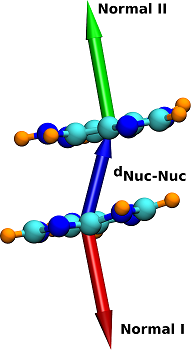
\includegraphics[width=\textwidth]{Introduction/Figures/Figure4.png}
    \caption[Representative structures for adenine self-assemblies over graphene]{(a) STM image of an epitaxially grown monolayer of adenine on graphite (001) with molecule positions indicated (size of the imaged area: 48$\angstrom$*32$\angstrom$; U = 1.0 V, I = 90 pA, constant current mode). (b) High-resolution STM constant-current image of alkyl-substituted adenine (A-C20) physisorbed onto a graphite surface from 1-phenyloctane solution (12.0 nm × 12.0 nm, V\textsubscript{bias} = 0.6 V, I\textsubscript{set} = 0.7 nA). (c) Model suggestion to characterize the packing in the STM image of panel b. (d) High-resolution STM constant-current image of A-C20 physisorbed onto a graphite surface from 1-phenyloctane solution (15.0 nm × 15.0 nm, V\textsubscript{bias} = 0.7 V, I\textsubscript{set} = 0.8 nA). (e) Model suggestion to characterize the packing in the STM image of panel d. Panel a is reprinted (figure) with permission from J. E. Freund, M. Edelwirth, P. Kro\"{b}el, and W. M. Heckl, Physical Review B, 55, 5394, 1997.\supercite{freund_structure_1997} Copyright 2023 by the American Physical Society. Panels b-d is Reprinted (adapted) with permission from ref \supercite{mu_temperature-dependent_2013}. Copyright 2023 American Chemical Society. }
    \label{fig:enter-label}
\end{figure}

Chi and coworkers investigated the self-assembly of a long alkyl-chain terminated adenine derivative on a HOPG surface as a function of temperature.\supercite{mu_temperature-dependent_2013} They employed in-situ STM imaging and ab-initio DFT calculations to characterize the self-assemblies observed in in-situ STM imaging. They observed the formation of two distinct forms ($\alpha$- and $\beta$-) of the self-assembly depending on the temperature and the interconversion between the two forms as a function of the temperature (Figure 1.4).

In a follow-up investigation, Chi and colleagues investigated the self-assembly of different long alkyl-chain terminated adenine molecules over a HOPG surface using STM imaging and DFT calculations.\supercite{wang_controlling_2014} They observed that the self-assemblies formed could be classified into two distinct groups ($\alpha$- and $\beta$-) depending on the formation temperature, and the structures could interchange between the forms as a function of the outside temperature. This observation aligns with the previous studies by them, where they investigated a chemically similar system under similar experimental conditions, with differences in sample preparation methods.\supercite{mu_temperature-dependent_2013} 

\paragraph{Guanine:} Spada and coworkers investigated the formation of self-assemblies in guanosine derivatives dipersed over an HOPG surface using STM imaging\supercite{gottarelli_self-assembly_2000}. They observed that the side chains remained flat on the graphene surface, and the self-assembled mono-layer consisted of two ribbon-like arrangements of guanine molecules interacting via hydrogen bonds.

Samor\`{i} and colleagues demonstrated the formation of self-assembled monolayers of N$^9$-substituted guanine molecules over a HOPG surface using STM imaging and subsequent DFT calculations.\supercite{ciesielski_nanopatterning_2010} They investigated the effect of side chain length on the observed self-assemblies at the HOPG - 1,2,4-trichlorobenzene interface. The authors observed the formation of distinct self-assemblies for varying side chain lengths, with the smallest alkyl chain molecule adopting and ribbon-like structure. In contrast, the larger ones progressively moved towards crystalline structures, stabilized via hydrogen bonding interactions.
\begin{figure}
    \centering
    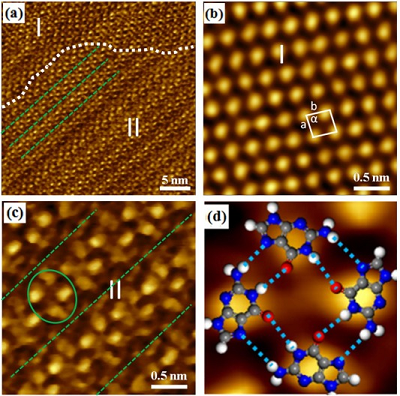
\includegraphics{Introduction/Figures/Figure6.png}
    \caption[Representative structures for guanine self-assemblies over graphene surface]{(a) Two G self-assembled networks in the water–HOPG interface (I = 0.85nA and V = -0.35 V). The white dashed line indicates the phase-separated boundary between structures I and II. (b) A high-resolution STM image of the structure of domain I (I = 0.75nA and V = -0.45 V). (c) An STM image of G-quartet structure II (I = 0.68nA and V = -0.53 V). The green circle surrounds a G-quartet. (d) The DFT-optimized structural model superimposed over a high-resolution STM image of the G-quartet. Figure adapted (reprinted) with permission from ref.\supercite{xu_directional_2021}. Copyright 2023 Elsevier.}
    \label{fig:enter-label}
\end{figure}

Samor\`{i} and colleagues demonstrated the inter-conversion between a ribbon-like guanine supramolecular structure and G4 quartets in N$^9$-alkylguanine molecules dispersed over a graphite surface\supercite{ciesielski_dynamers_2010}. They demonstrated that the structures can be inter-converted with the addition of potassium picrate, [2.2.2]cryptand and trifluromethanesulfonic acid (HTf), where the addition of potassium ions drives the conversion towards G4 quartets, and the addition of cryptand facilitating the back-conversion to ribbon-like structures. They were able to demonstrate the successive interconversions via STM imaging, where the observed transitions in the monolayer corresponded to the two states.

Li and coworkers investigated the formation of 2D self-assembled monolayers in guanine molecules dispersed over an HOPG surface using STM imaging\supercite{xu_directional_2021}. They observed that the guanine molecules self-assembled into two distinct strcutures, one resembling a linear structure, and other corresponding to a G4 quartet (Figure 1.5). They observed that the guanine quartets are connected via intermolecular hydrogen bonds, extending the observed 2D network into a line.

We note that multiple reports of guanosine-based self-assemblies are available in the literature\supercite{spada_guanosine-based_2008,xu_directional_2021,ciesielski_dynamers_2010,ciesielski_nanopatterning_2010,gottarelli_self-assembly_2000}, and the results seem to agree that the guanine molecules tend to self-assemble into one of the three forms: either into linear chains of guanine molecules, or into G4 quartets, or into a combination of these two forms. 

\paragraph{Cytosine:} Besenbacher and colleagues investigated the formation of 2D self-assembled monolayers dispersed over an HOPG surface using STM imaging and DFT calculations\supercite{xu_coadsorption_2006}. They observed that cytosine molecules self-assembled in 1D linear chains of cytosine molecules interacting via intermolecular hydrogen bonding interactions (Figure 1.6). From SCC-DFTB calculations, they identified that the 1D cytosine chain were formed from cytosine dimers interacting via symmetric hydrogen bonds between C2(O) and N1 atoms.
\begin{figure}
    \centering
    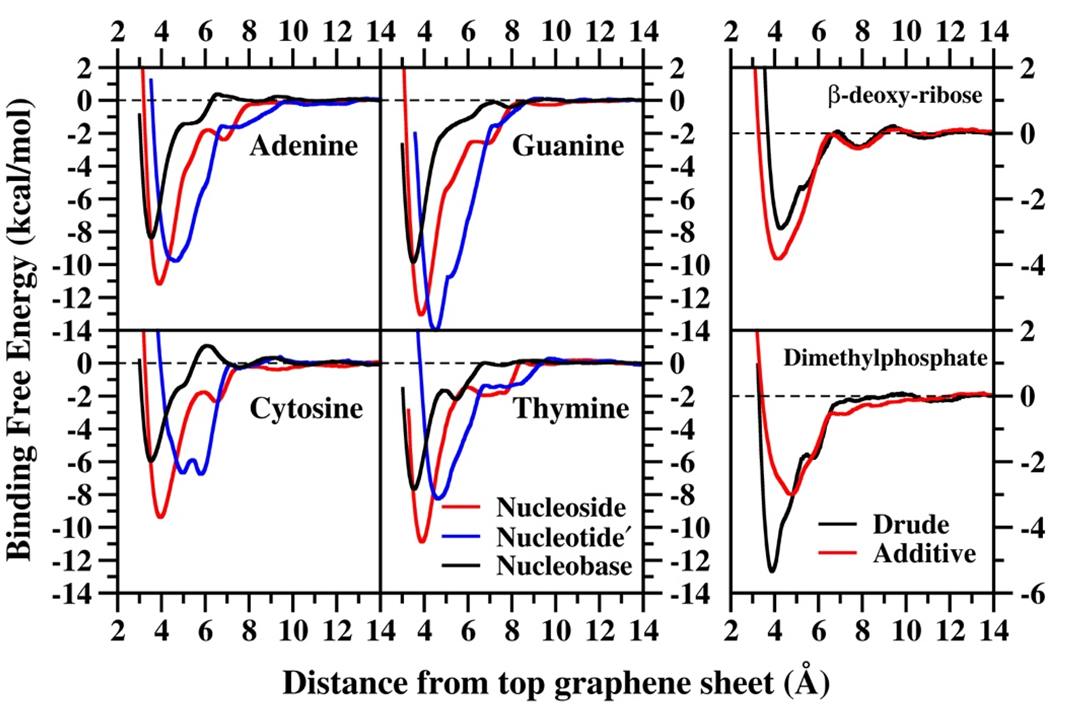
\includegraphics{Introduction/Figures/Figure11.png}
    \caption[Representative structures for cytosine self-assemblies over graphene surface]{(a) STM image of pure cytosine at water-HOPG interface (20*20  nm\textsuperscript{2};  scale bar, 5 nm; imaging tunneling current, 561.7 pA; tunneling bias, 770.3 mV). (b) Correlation-averaged zoom-in (5*5nm\textsuperscript{2}; scale bar, 1 nm). A unit cell is indicated. Reprinted (adpated) with permission from ref.\cite{xu_coadsorption_2006}. Copyright 2023 American Chemical Society. (c) STM image depicting the self-assembled networks formed by cytosine molecules at the water–HOPG interface (I = 0.74nA and V = -0.42 V). High-resolution STM images show (d) self-assembled networks formed by cytosine molecules (I = 0.78nA, V = -0.45 V). Figure adapted (reprinted) with permission from ref.\cite{xu_directional_2021}. Copyright 2023 Elsevier.}
    \label{fig:enter-label}
\end{figure}

Li and coworkers also investigated the formation of 2D self-assembled monolayes in cytosine molecules disperesed over an HOPG surface using STM imaging\supercite{xu_directional_2021}. They observed the formation of an ordered 2D self-assembled structure composed of parallel 1D chains, where individual cytosine molecules form four hydrogen bonds with two neighbors, forming a chainlike structure (Figure 1.6).